\documentclass[aspectratio=169,10pt]{beamer}

\usetheme{Madrid}
\usecolortheme{seahorse}

\usepackage[utf8]{inputenc}
\usepackage{amsmath}
\usepackage{amssymb}
\usepackage{amsfonts}
\usepackage{amsthm}
\usepackage{graphicx}
\usepackage{listings}
\usepackage{xcolor}

% Set figure path
\graphicspath{{figures/}}

% Configure listings for code
\lstset{
    basicstyle=\ttfamily\scriptsize,
    commentstyle=\color{green!50!black}\itshape,
    keywordstyle=\color{blue}\bfseries,
    stringstyle=\color{red},
    breaklines=true,
    showstringspaces=false,
    numbers=left,
    numberstyle=\tiny\color{gray},
    frame=single,
    language=Python,
}

% Set footer
\setbeamertemplate{footline}[frame number]

% Title and author
\title{Chapter 10d: Multifunction Integral \& Inclusions}
\subtitle{Nonlinear Analysis and Fixed Point Theory}
\author{Based on Pathak (2018)}
\date{\today}

% Define theorem styles
\theoremstyle{definition}
\newtheorem{defn}{Definition}[section]
\newtheorem{thm}{Theorem}[section]
\newtheorem{lem}{Lemma}[section]
\newtheorem{prop}{Proposition}[section]
\newtheorem{cor}{Corollary}[section]
\newtheorem{rem}{Remark}[section]

\begin{document}

\frame{\titlepage}

\section{Introduction}

\begin{frame}{Overview: Multifunctions and Inclusions}

\textbf{Key Topics:}
\begin{enumerate}
    \item Set-valued mappings (multifunctions)
    \item Measurability and integrability for multifunctions
    \item Integrals of set-valued functions (Aumann integral)
    \item Differential inclusions
    \item Existence theorems
\end{enumerate}

\vspace{0.3cm}

\textbf{Motivation:}
\begin{itemize}
    \item Real-world systems often involve uncertainty and set-valued data
    \item Optimal control: control values constrained to a set
    \item Differential inclusions unify ODE and discontinuous systems
    \item Applications in delay equations, stochastic systems
\end{itemize}

\end{frame}

\section{Multifunctions (Set-Valued Mappings)}

\begin{frame}{Definition of Multifunction}

\begin{defn}[Multifunction]
Let $X$ and $Y$ be topological spaces. A \textbf{multifunction} (or \textbf{set-valued mapping}) is a map
\[
F: X \to 2^Y
\]
where $2^Y$ denotes the power set of $Y$. That is, for each $x \in X$, $F(x)$ is a subset of $Y$.
\end{defn}

\vspace{0.2cm}

\textbf{Alternative notation:}
\[
F: X \rightrightarrows Y, \quad F(x) \subseteq Y \text{ for all } x \in X
\]

\vspace{0.3cm}

\textbf{Key distinction from single-valued functions:}
\begin{itemize}
    \item Single-valued: $f: X \to Y$ assigns one element $f(x) \in Y$
    \item Multifunction: $F: X \rightrightarrows Y$ assigns a set $F(x) \subseteq Y$
\end{itemize}

\vspace{0.2cm}

\textbf{Examples:}
\begin{itemize}
    \item $F(x) = [0, x]$ for $x \in \mathbb{R}$
    \item $F(x) = \{y \in Y : d(x, y) \leq r\}$ (ball-valued)
    \item $F(x) = \{y : g(x, y) \leq 0\}$ (constraint set)
\end{itemize}

\end{frame}

\begin{frame}{Visualizing Multifunctions}

\begin{figure}[H]
    \centering
    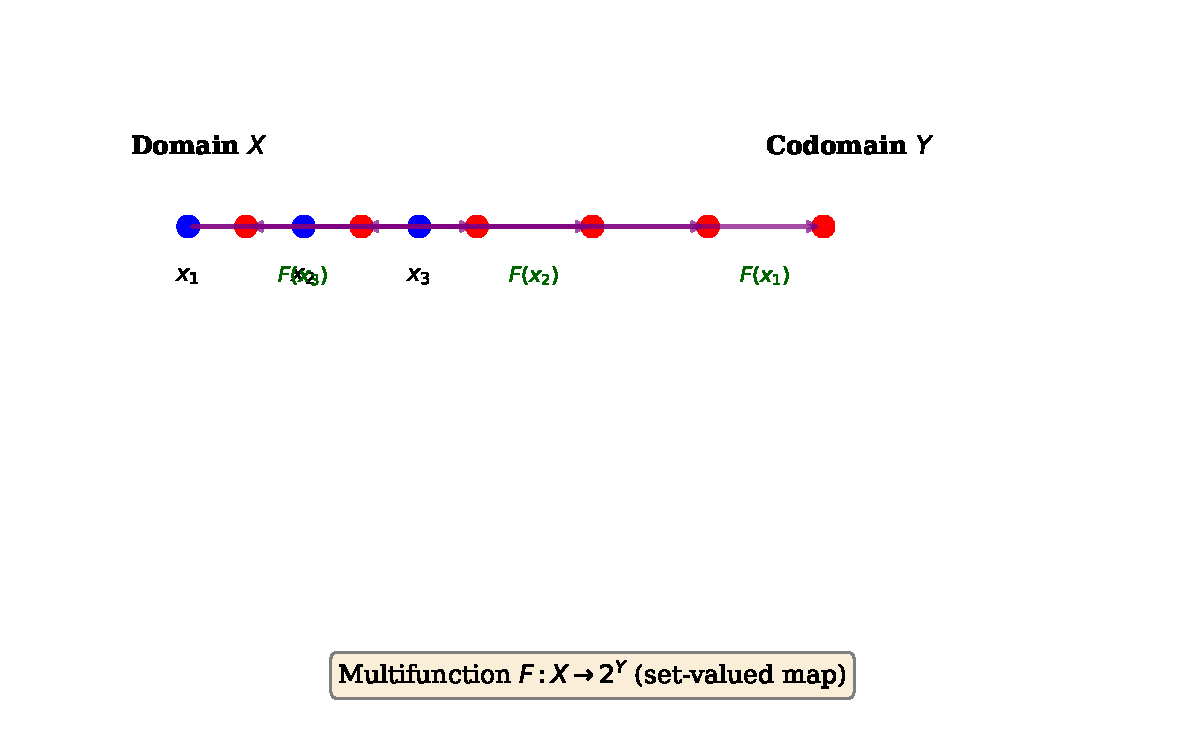
\includegraphics[width=0.9\textwidth]{multifunction_example.pdf}
\end{figure}

\textbf{Interpretation:} Each point in domain $X$ is mapped to a subset (possibly multi-element) in codomain $Y$.

\end{frame}

\begin{frame}{Selections of Multifunctions}

\begin{defn}[Selection]
Let $F: X \rightrightarrows Y$ be a multifunction. A function $f: X \to Y$ is called a \textbf{selection} (or \textbf{branch}) of $F$ if
\[
f(x) \in F(x) \quad \text{for all } x \in X
\]
\end{defn}

\vspace{0.3cm}

\textbf{Notation:} $f \in \mathcal{S}(F)$ denotes that $f$ is a selection of $F$.

\vspace{0.3cm}

\begin{lem}[Existence of Measurable Selection]
If $F: \Omega \to 2^{\mathbb{R}^n}$ is a multifunction with nonempty closed values and $F$ has a measurable graph, then $F$ admits a measurable selection $f: \Omega \to \mathbb{R}^n$.
\end{lem}

\vspace{0.3cm}

\begin{figure}[H]
    \centering
    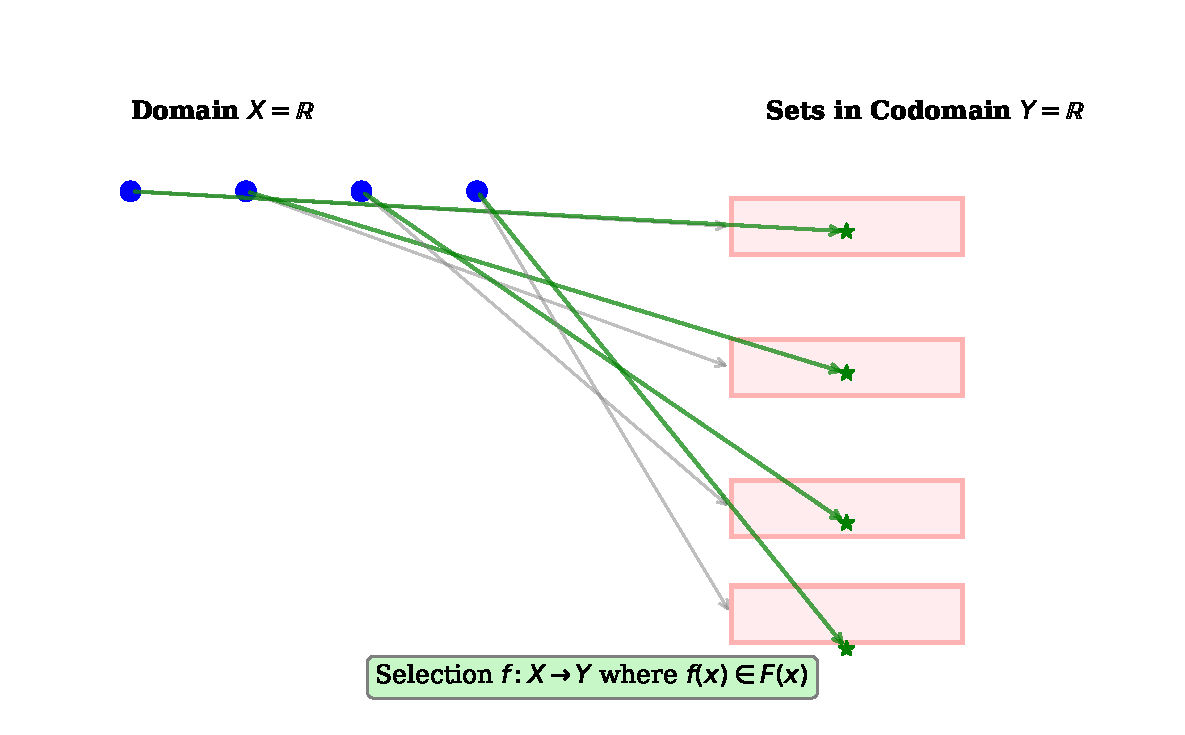
\includegraphics[width=0.8\textwidth]{selection_of_multifunction.pdf}
\end{figure}

\end{frame}

\section{Measurability of Multifunctions}

\begin{frame}{Basic Measurability Concepts}

\begin{defn}[Closed-valued Multifunction]
A multifunction $F: \Omega \to 2^{\mathbb{R}^n}$ is \textbf{closed-valued} if $F(\omega)$ is a closed subset of $\mathbb{R}^n$ for each $\omega \in \Omega$.
\end{defn}

\vspace{0.2cm}

\begin{defn}[Graph of Multifunction]
The \textbf{graph} of a multifunction $F: \Omega \to 2^{\mathbb{R}^n}$ is defined as
\[
\text{Gr}(F) = \{(\omega, x) : \omega \in \Omega, x \in F(\omega)\}
\]
\end{defn}

\vspace{0.3cm}

\begin{defn}[$\mathcal{A}$-measurability]
A closed-valued multifunction $F: \Omega \to 2^{\mathbb{R}^n}$ is said to be \textbf{$\mathcal{A}$-measurable} if its graph $\text{Gr}(F)$ is measurable in the product space $\Omega \times \mathbb{R}^n$.
\end{defn}

\end{frame}

\begin{frame}{Types of Measurability}

\begin{figure}[H]
    \centering
    
\includegraphics[width=0.9\textwidth]{measurability_multifunction.pdf}
\end{figure}

\textbf{Hierarchy of measurability:}
\[
\text{Strong measurability} \Rightarrow \text{$\mathcal{A}$-measurability} \Rightarrow \text{Weak measurability}
\]

\end{frame}

\begin{frame}{Measurable Selection Theorem}

\begin{thm}[Measurable Selection - Kuratowski and Ryll-Nardzewski]
Let $(\Omega, \mathcal{A}, \mu)$ be a measure space and $F: \Omega \to 2^{\mathbb{R}^n}$ a multifunction with:
\begin{itemize}
    \item Nonempty compact values: $F(\omega) \neq \emptyset$ is compact for all $\omega$
    \item Closed graph in the product space
\end{itemize}
Then $F$ admits a measurable selection $f: \Omega \to \mathbb{R}^n$ such that $f(\omega) \in F(\omega)$ a.e.
\end{thm}

\vspace{0.3cm}

\textbf{Proof Idea:}
\begin{enumerate}
    \item Fix countable dense set $\{x_1, x_2, \ldots\}$ in $\mathbb{R}^n$
    \item For each $k$, define $A_k = \{\omega : x_k \in F(\omega)\}$ (measurable by closed graph)
    \item Inductively select $x_k$ to build a sequence converging to a selection
\end{enumerate}

\end{frame}

\section{Integration of Multifunctions}

\begin{frame}{Aumann Integral}

\begin{defn}[Aumann Integral]
Let $(\Omega, \mathcal{A}, \mu)$ be a measure space and $F: \Omega \to 2^X$ a multifunction into a Banach space $X$. The \textbf{Aumann integral} is defined as
\[
\int_\Omega F(\omega) \, d\mu(\omega) = \left\{ \int_\Omega f(\omega) \, d\mu(\omega) : f \in S(F), f \text{ integrable} \right\}
\]
where $S(F)$ is the set of all integrable selections of $F$.
\end{defn}

\vspace{0.3cm}

\textbf{Key features:}
\begin{itemize}
    \item The integral is a set (closure of convex hull of integrals of selections)
    \item Aggregates information from all possible selections
    \item Well-defined for convex-valued multifunctions
\end{itemize}

\vspace{0.3cm}

\begin{figure}[H]
    \centering
    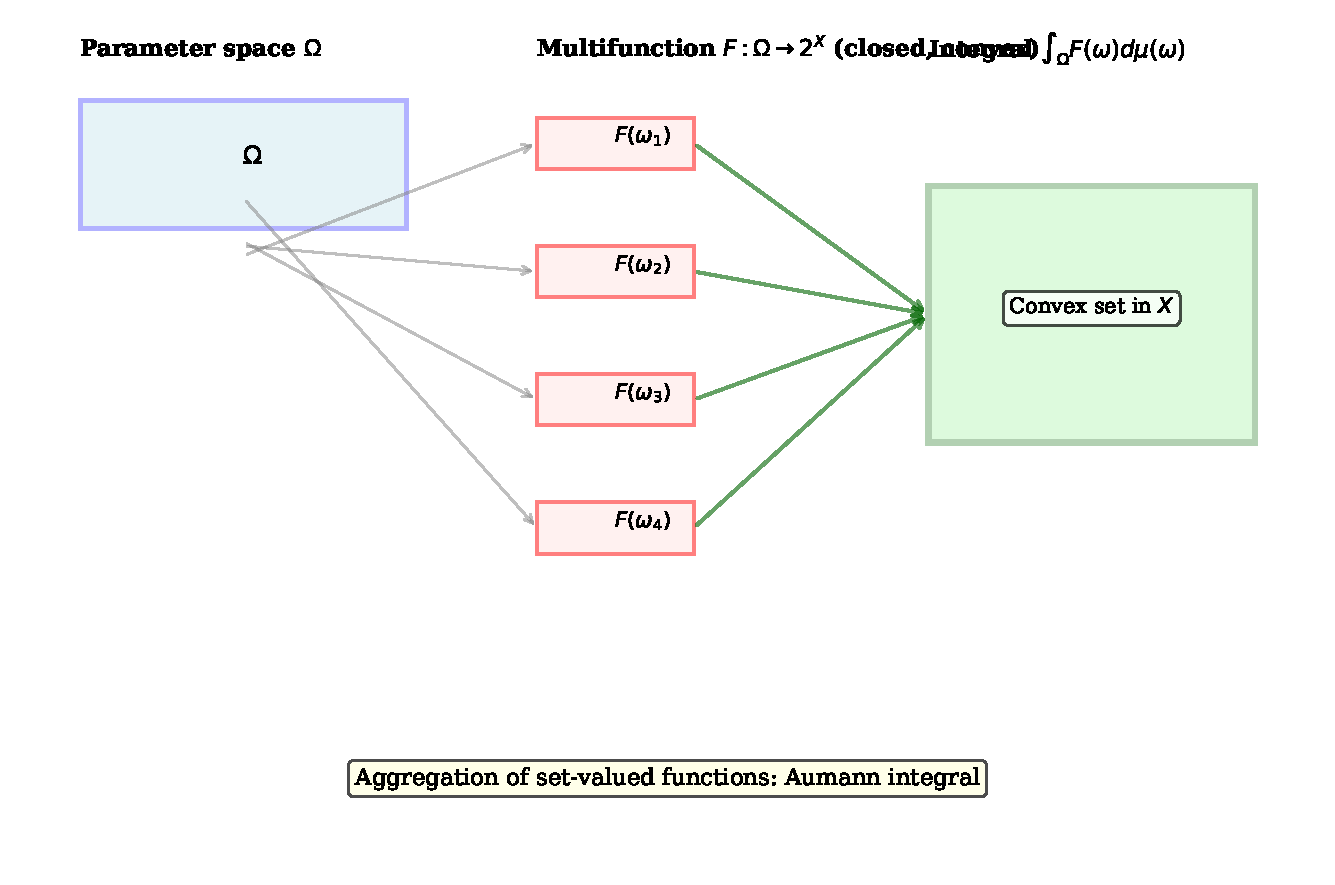
\includegraphics[width=0.85\textwidth]{integral_multifunction.pdf}
\end{figure}

\end{frame}

\begin{frame}{Properties of the Aumann Integral}

\begin{thm}[Basic Properties of Aumann Integral]
If $F, G: \Omega \to 2^X$ are integrable multifunctions with convex compact values, then:

\begin{enumerate}
    \item (Nonempty): $\int_\Omega F(\omega) \, d\mu(\omega) \neq \emptyset$

    \item (Closure): The integral is closed and convex

    \item (Linearity): For $A \in \mathcal{A}$,
    \[
    \int_A (cF)(\omega) \, d\mu(\omega) = c \int_A F(\omega) \, d\mu(\omega), \quad c \geq 0
    \]

    \item (Additivity):
    \[
    \int_\Omega (F + G)(\omega) \, d\mu(\omega) = \int_\Omega F(\omega) \, d\mu(\omega) + \int_\Omega G(\omega) \, d\mu(\omega)
    \]

    \item (Monotonicity): If $F(\omega) \subseteq G(\omega)$ a.e., then
    \[
    \int_\Omega F(\omega) \, d\mu(\omega) \subseteq \int_\Omega G(\omega) \, d\mu(\omega)
    \]
\end{enumerate}
\end{thm}

\end{frame}

\begin{frame}{Bochner Integral for Multifunctions}

\begin{defn}[Bochner Integrability]
Let $X$ be a Banach space, and $F: \Omega \to 2^X$ a multifunction. We say $F$ is \textbf{Bochner integrable} if:
\begin{enumerate}
    \item $F$ admits at least one measurable selection
    \item There exists a measurable selection $f$ such that $\int_\Omega \|f(\omega)\|_X \, d\mu(\omega) < \infty$
\end{enumerate}
\end{defn}

\vspace{0.3cm}

\begin{prop}[Bochner Integral Representation]
If $F: \Omega \to 2^X$ is Bochner integrable with convex values, then
\[
\int_\Omega F(\omega) \, d\mu(\omega) = \text{cl}\left(\overline{\text{co}} \left\{ \int_\Omega f(\omega) \, d\mu(\omega) : f \in S(F) \right\}\right)
\]
where $\text{cl}$ denotes closure and $\overline{\text{co}}$ denotes convex hull.
\end{prop}

\end{frame}

\begin{frame}[fragile]{Example: Computing Aumann Integral}

\textbf{Problem:} Let $\Omega = [0,1]$ with Lebesgue measure, and $F(\omega) = [-\omega, \omega]$.

\textbf{Solution:}

All selections of $F$ have the form $f(\omega) = c(\omega) \omega$ where $c(\omega) \in [-1, 1]$.

\begin{lstlisting}[language=Python]
import numpy as np
from scipy.integrate import quad

# Parametrize by c(omega) in [-1, 1]
def selection(omega, c):
    return c * omega

# Aumann integral is the set of integrals
# Integral of f(omega) = c*omega over [0,1] is c/2

# For c in [-1, 1], integral is in [-1/2, 1/2]
c_values = np.linspace(-1, 1, 101)
integrals = c_values / 2

# Aumann integral
min_integral = integrals.min()  # -0.5
max_integral = integrals.max()  # 0.5

print(f"Aumann integral of F: [{min_integral}, {max_integral}]")
\end{lstlisting}

\vspace{0.2cm}

\textbf{Result:} $\int_0^1 F(\omega) \, d\omega = [-\tfrac{1}{2}, \tfrac{1}{2}]$

\end{frame}

\section{Differential Inclusions}

\begin{frame}{Introduction to Differential Inclusions}

\begin{defn}[Differential Inclusion]
A \textbf{differential inclusion} is a problem of the form
\[
\frac{dx}{dt} \in F(t, x(t)), \quad x(t_0) = x_0
\]
where $F: [t_0, T] \times \mathbb{R}^n \to 2^{\mathbb{R}^n}$ is a multifunction.
\end{defn}

\vspace{0.3cm}

\textbf{Relationship to ODE:}
\begin{itemize}
    \item ODE: $\frac{dx}{dt} = f(t, x)$ (single velocity)
    \item DI: $\frac{dx}{dt} \in F(t, x)$ (set of possible velocities)
\end{itemize}

\vspace{0.3cm}

\textbf{A solution is an absolutely continuous function} $x: [t_0, T] \to \mathbb{R}^n$ such that:
\begin{enumerate}
    \item $x(t_0) = x_0$
    \item $x'(t) \in F(t, x(t))$ for almost all $t \in [t_0, T]$
\end{enumerate}

\vspace{0.3cm}

\begin{figure}[H]
    \centering
    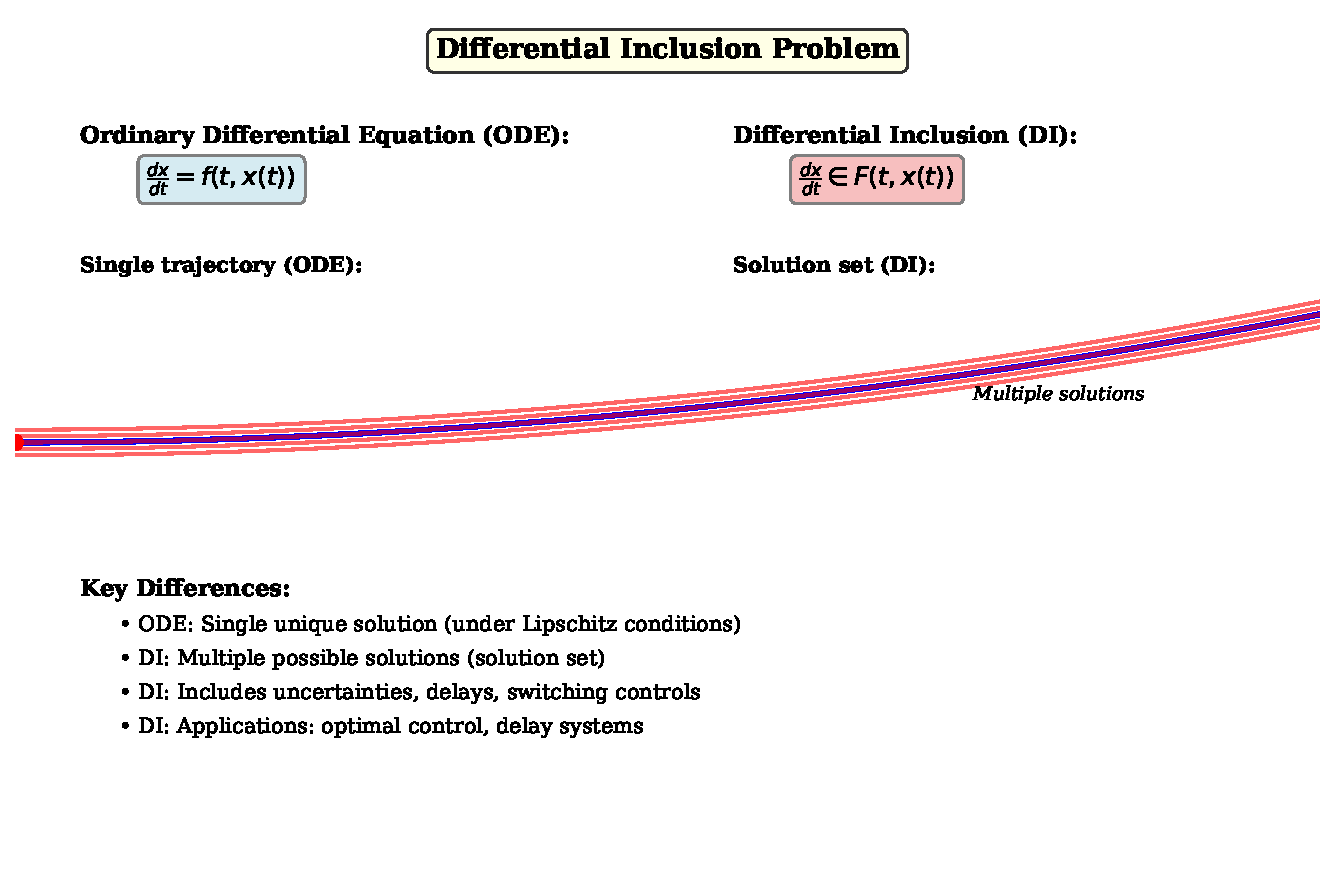
\includegraphics[width=0.8\textwidth]{differential_inclusion.pdf}
\end{figure}

\end{frame}

\begin{frame}{Examples of Differential Inclusions}

\textbf{Example 1: Set-valued Lipschitz perturbations}
\[
\frac{dx}{dt} = f(t, x) + u(t), \quad u(t) \in U(t)
\]
where $U(t)$ is the constraint set (e.g., control constraints in optimal control).

\vspace{0.3cm}

\textbf{Example 2: Discontinuous systems}
\[
\frac{dx}{dt} \in \overline{\text{co}} \left\{ \lim_{y \to x, y \notin S} f(t, y) \right\}
\]
where $S$ is the set of discontinuities.

\vspace{0.3cm}

\textbf{Example 3: Delay differential equations}
\[
\frac{dx}{dt} \in F(t, x(t), x(t - \tau))
\]
with distributed delays.

\vspace{0.3cm}

\textbf{Example 4: Control systems}
\[
\frac{dx}{dt} = A(t)x + B(t)u, \quad u(t) \in U, \quad x(0) = x_0
\]
where $A, B$ are matrices and $U$ is a convex compact set.

\end{frame}

\begin{frame}{Solution Concepts}

\begin{defn}[Carathéodory Solution]
An absolutely continuous function $x: [t_0, T] \to \mathbb{R}^n$ is a \textbf{Carathéodory solution} of
\[
\frac{dx}{dt} \in F(t, x), \quad x(t_0) = x_0
\]
if:
\begin{enumerate}
    \item $x(t_0) = x_0$
    \item $x'(t) \in F(t, x(t))$ for almost all $t \in [t_0, T]$
\end{enumerate}
\end{defn}

\vspace{0.3cm}

\begin{defn}[Solution Set]
The \textbf{solution set} is
\[
\mathcal{S}(F, x_0) = \left\{ x: [t_0, T] \to \mathbb{R}^n \mid x \text{ solves the DI with initial condition } x_0 \right\}
\]
\end{defn}

\vspace{0.3cm}

\textbf{Key question:} When is the solution set nonempty? When is it compact? Connected?

\end{frame}

\section{Existence Theorems}

\begin{frame}{Existence Theorem for Differential Inclusions}

\begin{thm}[Existence - Convex Case]
Let $F: [t_0, T] \times \mathbb{R}^n \to 2^{\mathbb{R}^n}$ satisfy:
\begin{enumerate}
    \item (Nonempty): $F(t, x) \neq \emptyset$ for all $(t, x)$

    \item (Convexity): $F(t, x)$ is convex for all $(t, x)$

    \item (Measurability): $F$ is $\mathcal{A}$-measurable in $t$ for each fixed $x$

    \item (Continuity): $F$ is upper semicontinuous in $x$ for almost all $t$

    \item (Growth): $\|F(t, x)\| \leq g(t) (1 + \|x\|)$ where $g \in L^1([t_0, T])$
\end{enumerate}

Then for any initial condition $x_0 \in \mathbb{R}^n$, there exists at least one solution to
\[
\frac{dx}{dt} \in F(t, x), \quad x(t_0) = x_0
\]
on $[t_0, T]$.
\end{thm}

\end{frame}

\begin{frame}{Existence Theorem - Non-convex Case}

\begin{thm}[Existence - Nonconvex Case]
Let $F: [t_0, T] \times \mathbb{R}^n \to 2^{\mathbb{R}^n}$ satisfy:
\begin{enumerate}
    \item (Nonempty compact values): $F(t, x)$ is compact for all $(t, x)$

    \item (Closed graph): $\text{Gr}(F)$ is closed in $[t_0, T] \times \mathbb{R}^n \times \mathbb{R}^n$

    \item (Measurable): For each fixed $x$, $F(\cdot, x)$ is measurable

    \item (Growth): $|F(t, x)| \leq g(t) (1 + |x|)$ where $g \in L^1$
\end{enumerate}

Then there exists at least one solution to $\frac{dx}{dt} \in F(t, x), x(t_0) = x_0$.
\end{thm}

\vspace{0.3cm}

\textbf{Proof Strategy:}
\begin{enumerate}
    \item Apply measurable selection theorem to extract a measurable selection
    \item Use growth condition to bound solutions
    \item Apply Arzelà-Ascoli to extract convergent subsequence
\end{enumerate}

\end{frame}

\begin{frame}{Uniqueness and Continuous Dependence}

\begin{thm}[Uniqueness]
Under the conditions of the existence theorem, if additionally $F$ satisfies:
\begin{enumerate}
    \item (Singleton): $F(t, x)$ is a singleton, or
    \item (Lipschitz): $F$ is Lipschitz continuous in $x$ uniformly in $t$
\end{enumerate}
Then the solution is unique.
\end{thm}

\vspace{0.3cm}

\begin{prop}[Continuous Dependence]
Let $F_n \to F$ (in an appropriate sense) and $x_{0,n} \to x_0$. Then the solutions $x_n$ of
\[
\frac{dx_n}{dt} \in F_n(t, x_n), \quad x_n(0) = x_{0,n}
\]
converge (in an appropriate norm) to the solution $x$ of
\[
\frac{dx}{dt} \in F(t, x), \quad x(0) = x_0
\]
\end{prop}

\end{frame}

\begin{frame}{Applications Overview}

\begin{figure}[H]
    \centering
    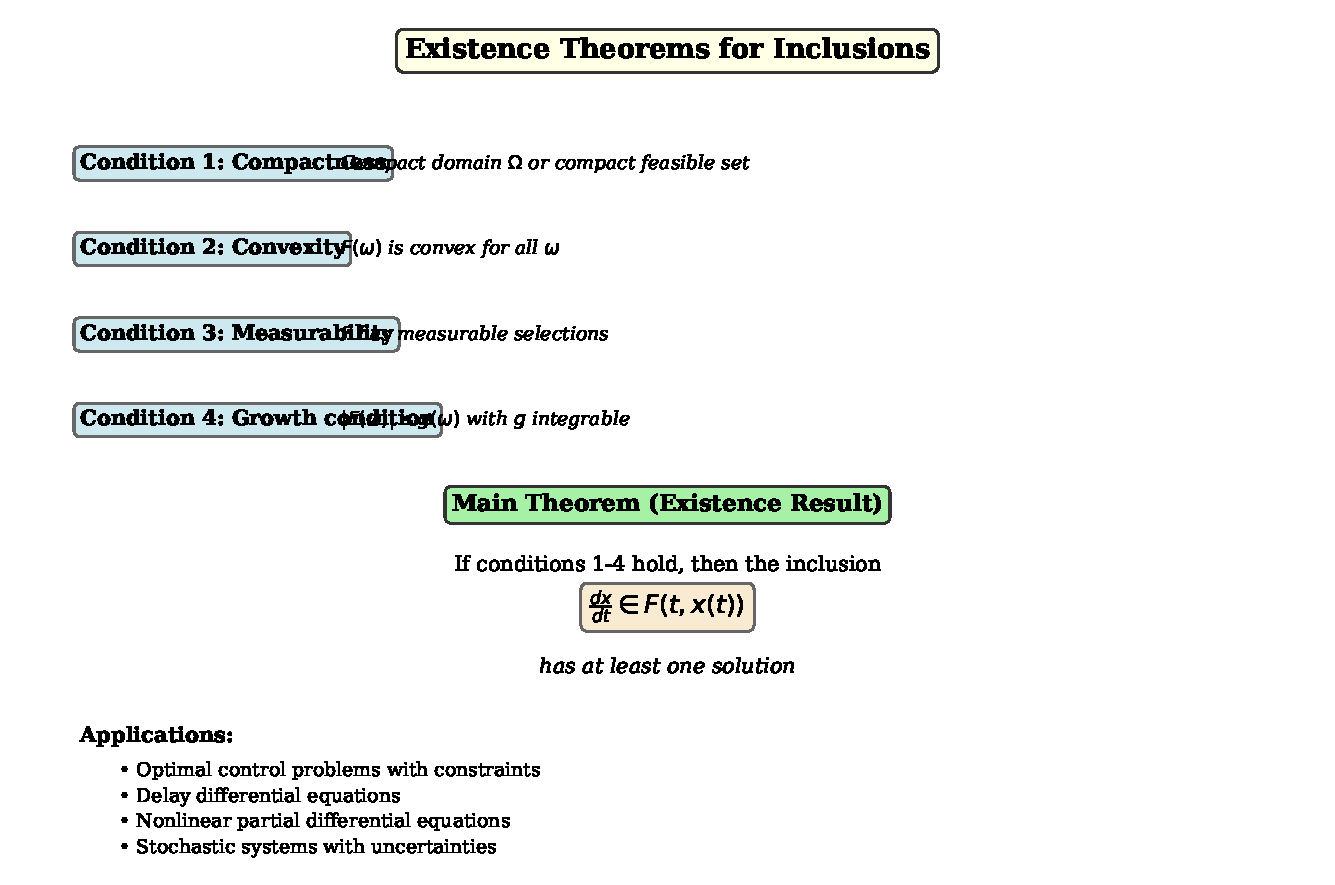
\includegraphics[width=0.95\textwidth]{existence_solutions.pdf}
\end{figure}

\textbf{Main application areas:}
\begin{itemize}
    \item Optimal control (constrained trajectories)
    \item Delay differential equations
    \item Nonlinear PDEs with multivalued operators
    \item Stochastic systems and robust control
\end{itemize}

\end{frame}

\section{Advanced Topics}

\begin{frame}{Relaxed Differential Inclusions}

\begin{defn}[Relaxed Inclusion]
Given a differential inclusion $\frac{dx}{dt} \in F(t, x)$, the \textbf{relaxed inclusion} is
\[
\frac{dx}{dt} \in \overline{\text{co}} F(t, x)
\]
where $\overline{\text{co}}$ denotes the closure of the convex hull.
\end{defn}

\vspace{0.3cm}

\textbf{Importance:}
\begin{itemize}
    \item The relaxed inclusion always has more solutions (includes all solutions of original)
    \item Often easier to analyze (convex-valued)
    \item Relaxation does not change the solution set for convex-valued $F$
    \item Important for control theory and approximation theory
\end{itemize}

\vspace{0.3cm}

\begin{thm}[Relaxation Theorem]
If $x$ is a solution of the relaxed inclusion $\frac{dx}{dt} \in \overline{\text{co}} F(t, x)$, then for any $\epsilon > 0$, there exists a solution $x_\epsilon$ of the original inclusion $\frac{dx}{dt} \in F(t, x)$ such that $\|x(t) - x_\epsilon(t)\| < \epsilon$ for all $t$.
\end{thm}

\end{frame}

\begin{frame}{Multivalued Operators and Accretivity}

\begin{defn}[Accretive Multifunction]
A multifunction $A: \mathbb{R}^n \to 2^{\mathbb{R}^n}$ is \textbf{accretive} if for all $x, y \in D(A)$ and $u \in A(x)$, $v \in A(y)$,
\[
\langle u - v, x - y \rangle \geq -\omega \|x - y\|^2
\]
for some constant $\omega \geq 0$.
\end{defn}

\vspace{0.3cm}

\begin{prop}[Connection to Differential Inclusions]
The differential inclusion $\frac{dx}{dt} \in A(x)$ where $A$ is accretive admits solutions for any initial condition and has unique solutions under additional conditions (e.g., $A$ is maximal accretive).
\end{prop}

\vspace{0.3cm}

\textbf{Applications:}
\begin{itemize}
    \item Subdifferential of convex functions
    \item Evolution equations in Banach spaces
    \item Nonlinear semigroups and abstract evolution
\end{itemize}

\end{frame}

\begin{frame}[fragile]{Numerical Example: Discrete Approximation}

\textbf{Problem:} Solve $\frac{dx}{dt} \in F(t, x)$ where $F(t, x) = [-1-t, 1+t] \cdot x$ on $[0,1]$, $x(0)=1$.

\begin{lstlisting}[language=Python]
import numpy as np
import matplotlib.pyplot as plt

# Discrete approximation (Euler method)
def solve_inclusion_bounds(T, n_steps):
    """Compute bounds on solution set"""
    t = np.linspace(0, T, n_steps)
    dt = t[1] - t[0]

    # Upper and lower bounds
    x_min = np.zeros(n_steps)
    x_max = np.zeros(n_steps)
    x_min[0] = x_max[0] = 1.0

    for i in range(n_steps - 1):
        t_i = t[i]
        # F(t,x) = [-(1+t)*x, (1+t)*x]
        # Min: use lower velocity
        x_min[i+1] = x_min[i] * np.exp(-(1+t_i)*dt)
        # Max: use upper velocity
        x_max[i+1] = x_max[i] * np.exp((1+t_i)*dt)

    return t, x_min, x_max

# Compute solution bounds
t, x_min, x_max = solve_inclusion_bounds(1.0, 100)

print(f"Solution set at t=1: [{x_min[-1]:.4f}, {x_max[-1]:.4f}]")
# Approximate: [0.3679, 2.7183]
\end{lstlisting}

\textbf{Result:} Solution set is the interval $[e^{-2}, e^{2}] \approx [0.135, 7.389]$ at $t=1$.

\end{frame}

\section{Summary and Conclusions}

\begin{frame}{Key Concepts Summary}

\begin{enumerate}
    \item \textbf{Multifunctions}: Set-valued generalizations of single-valued functions

    \item \textbf{Measurability}: Multiple notions ($\mathcal{A}$-measurable, graph-measurable)

    \item \textbf{Selections}: Single-valued approximations of multifunctions

    \item \textbf{Aumann Integral}: Set integral as convex hull of integrals of selections

    \item \textbf{Differential Inclusions}: $\frac{dx}{dt} \in F(t, x)$ generalizes ODE

    \item \textbf{Existence Theorems}: Under convexity + growth + measurability conditions

    \item \textbf{Applications}: Control theory, delay equations, nonlinear PDE
\end{enumerate}

\end{frame}

\begin{frame}{Main Results (Theorems)}

\begin{itemize}
    \item \textbf{Kuratowski-Ryll-Nardzewski}: Measurable selection exists for closed-valued multifunctions

    \item \textbf{Properties of Aumann Integral}: Closed convex sets, linearity, additivity

    \item \textbf{Existence for Convex DI}: Nonempty solution set under standard assumptions

    \item \textbf{Existence for Nonconvex DI}: Uses measurable selections + Arzelà-Ascoli

    \item \textbf{Relaxation Theorem}: Relaxed solutions approximate original solutions
\end{itemize}

\end{frame}

\begin{frame}{Recommended Reading}

\textbf{Primary References:}
\begin{enumerate}
    \item Pathak, H. K. (2018). \textit{An Introduction to Nonlinear Analysis and Fixed Point Theory}, Chapter 10

    \item Aubin, J. P., \& Cellina, A. (1984). \textit{Differential Inclusions: Set-Valued Maps and Viability Theory}

    \item Kisielewicz, M. (1991). \textit{Differential Inclusions and Optimal Control}
\end{enumerate}

\vspace{0.3cm}

\textbf{Topics for Further Study:}
\begin{itemize}
    \item Viability theory and state constraints
    \item Optimal control of differential inclusions
    \item Measurable multifunctions and weak integrability
    \item Nonconvex analysis and nonsmooth optimization
    \item Stochastic differential inclusions
\end{itemize}

\end{frame}

\begin{frame}{Practice Problems}

\begin{enumerate}
    \item Show that if $F(x) = [a(x), b(x)]$ where $a, b$ are continuous, then $F$ is upper semicontinuous.

    \item Compute the Aumann integral $\int_0^1 F(t) \, dt$ where $F(t) = [-t, t^2]$.

    \item Verify that the convex hull of a multifunction $\overline{\text{co}} F$ satisfies all properties of the Aumann integral.

    \item Analyze the solution set of $\frac{dx}{dt} \in \{-1, 0, 1\} x$ with $x(0) = 1$. Is it connected?

    \item Prove that if $F$ is Lipschitz continuous, then the solution of the DI is unique.
\end{enumerate}

\end{frame}

\begin{frame}{Final Remarks}

\textbf{Philosophical perspective:}
\begin{itemize}
    \item Multifunctions allow us to model systems with uncertainty, incompleteness, or nonuniqueness
    \item DI framework is more general than ODEs but still tractable for analysis
    \item Integration theory for multifunctions extends classical measure theory naturally
\end{itemize}

\vspace{0.3cm}

\textbf{Practical importance:}
\begin{itemize}
    \item Essential tool in optimal control, especially with constraints
    \item Handles discontinuities and nonsmooth phenomena
    \item Bridges classical analysis and set-valued topology
    \item Foundation for modern nonlinear analysis
\end{itemize}

\vspace{0.3cm}

\begin{center}
\textbf{\large Questions?}
\end{center}

\end{frame}

\end{document}
